%%%%%%%%%%%%%%%%%%%% author.tex %%%%%%%%%%%%%%%%%%%%%%%%%%%%%%%%%%%
%
%%%%%%%%%%%%%%%% Springer %%%%%%%%%%%%%%%%%%%%%%%%%%%%%%%%%%

\title*{A (nearly) full analysis of a GP run}
% Use \titlerunning{Short Title} for an abbreviated version of
% your contribution title if the original one is too long
\author{Nicholas Freitag McPhee, Maggie M. Casale, Mitchell Finzel, Thomas Helmuth and Lee Spector}
% Use \authorrunning{Short Title} for an abbreviated version of
% your contribution title if the original one is too long
\institute{Nicholas Freitag McPhee, Maggie M. Casale and Mitchell Finzel \at University of Minnesota, Morris; Morris, MN USA
\and Thomas Helmuth \at Washington and Lee University, Lexington, VA USA
\and Lee Spector \at Hampshire College, Amerherst, MA USA}

\maketitle

\abstract{We analyze the key events in a GP run!}

\begin{keywords}
	genetic programming, PushGP, ancestry graph, lineage, inheritance
\end{keywords}
\index{genetic programming}
\index{PushGP}
\index{ancestry graph}
\index{lineage}
\index{inheritance}
\\
\section{Introduction}
\label{sec:introduction}

Motivate the work!

\section{Plush genomes and PushGP operators}
\label{sec:background}

\todo{I'm hoping we can crib most of this section from previous works, e.g.,
	Tom's dissertation, the Plush GPTP paper, and other papers.}

We'll need to (quickly) outline the key elements of the Plush genome, including
the \texttt{:instruction} and \texttt{:close} components. (This run didn't use the
\texttt{:silent} component, so we can ignore that.)

We'll also need to describe the genetic operators used in PushGP/Clojush.

And replace-space-with-newline.

And simplification.

%Use the standard \verb|equation| environment to typeset your equations, e.g.
%%
%\begin{equation}
%a \times b = c\;,
%\end{equation}
%%
%however, for multiline equations we recommend to use the \verb|eqnarray| environment.
%\begin{eqnarray}
%a \times b = c \nonumber\\
%\vec{a}   \vec{b}=\vec{c}
%\label{eq:01}
%\end{eqnarray}

\section{Analysis of a run}

\begin{itemize}
	\item Describe the basics of the run (length, etc.).
\end{itemize}

Then work backwards from the winner back through to the start of the run.

\subsection{Full ancestry graph}

Figure~\ref{fig:run0Labelled} shows the full ancestry tree of the 13 successful 
individuals in this run. Each individual in the run is represented with a
rectangle containing an identifier of the form \texttt{X:Y}, where \texttt{X}
is the generation number, and \texttt{Y} is an arbitrary individual number
within that generation. Each generation is a row, with the initial random
individuals being at the top and the 13 successful individuals at the bottom.

\begin{sidewaysfigure}[tb!p] %[b] sets the image at the bottom of the page; t = top, b = bottom, h = here%
	% \sidecaption
	% Use the relevant command for your figure-insertion program
	% to insert the figure file.
	% For example, with the graphicx style use
	\begin{center}
		\vspace{0.6\columnwidth}
		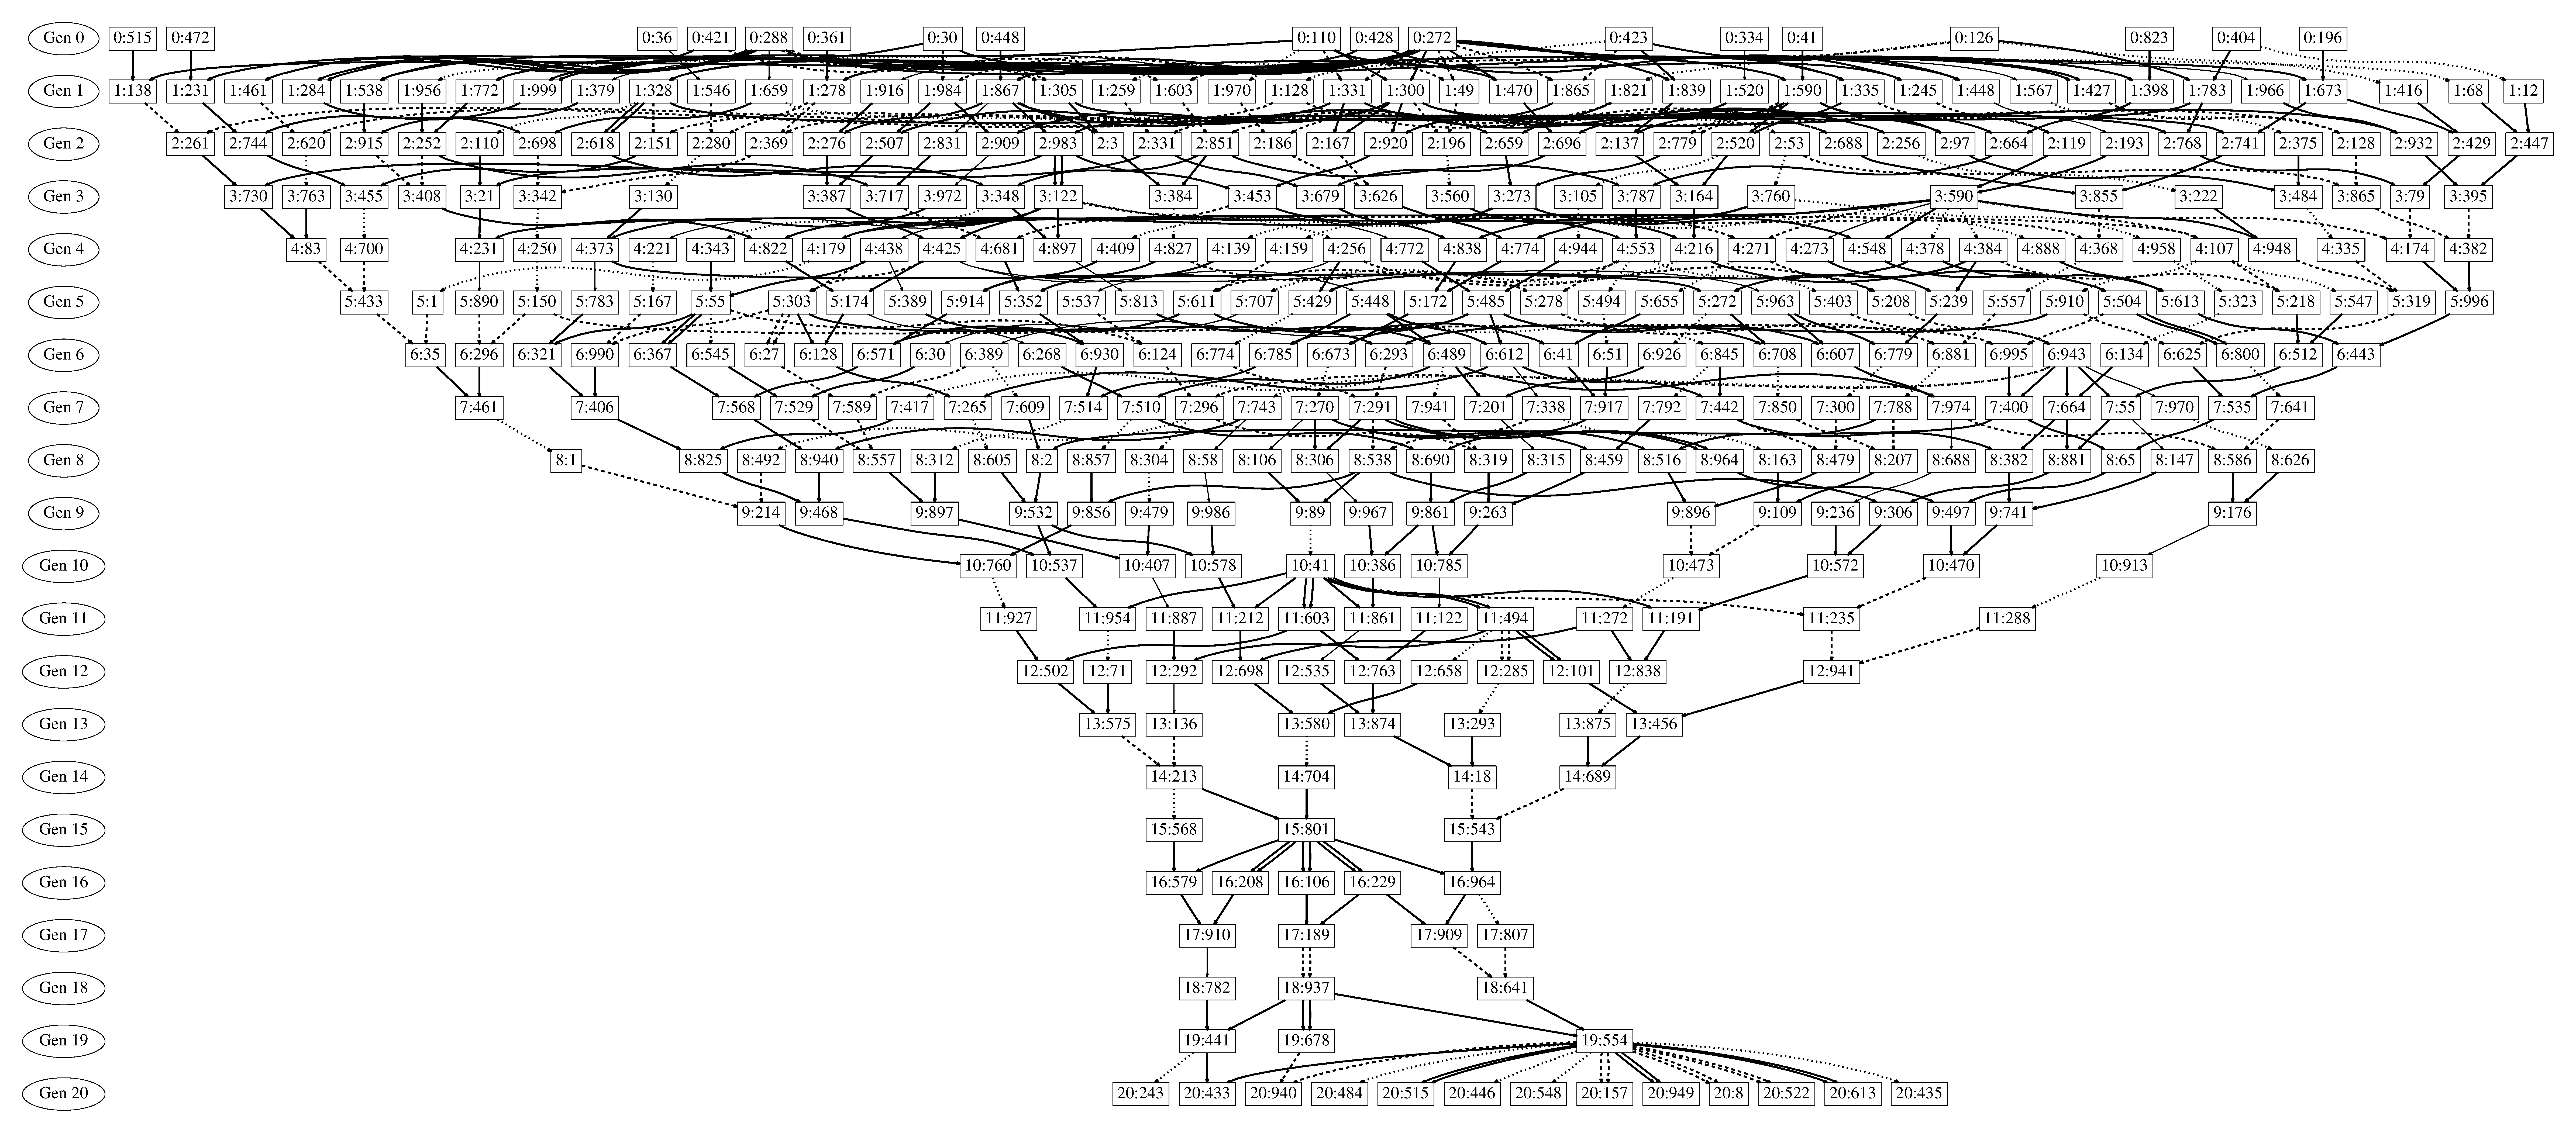
\includegraphics[width=\columnwidth]{../figures/run0_GPTP_2_font_30}
	\end{center}
	\caption{The labelled run.}
	\label{fig:run0Labelled}       % Give a unique label
\end{sidewaysfigure}

The edges indicate the particular genetic operator used to construct a child
as follows:
\begin{itemize}
	\item Thick black lines: alternation and uniform mutation
	\item Dashed: alternation
	\item Dotted: uniform mutation
	\item Thin black lines: uniform close mutation
\end{itemize}

This graph includes \emph{every} individual in this run that was an 
ancestor of one of the winners, i.e., every individual that could possibly have 
contributed genetic material to one of the winners. Note, however, that not
all these individuals actually contributed any genetic material to those
solutions. There are, for example, cases where one of the parents actually
contributed no material in a recombination (alternation) event, and cases where
a parent did contribute some genetic material, but that material was later
removed or replaced in subsequent mutations or recombinations. 

Conversely, while the individuals not represented in this graph are
guaranteed to have not contributed to the genetics of the successful
individual, they might have still had some substantial impact on the
run's overall dynamics. The presence of those individuals and their
error vectors could certainly affect lexicase selection's choice of parents,
for example, which could substantially impact the dynamics.

\subsection{Filtered ancestry graph}

Despite the short length of this run, and the restriction to just displaying
ancestors of successful individuals, Figure~\ref{fig:run0Labelled} still
contains 394 nodes and 629 edges, making it difficult to analyze in full.
Figure~\ref{fig:run0Filtered} is a version of the same graph that further
filters the ancestry tree, attempting the highlight the individuals that
are most likely to have contributed a significant amount of genetic material
to the solutions.

\begin{figure}[tb!p] %[b] sets the image at the bottom of the page; t = top, b = bottom, h = here%
	% \sidecaption
	% Use the relevant command for your figure-insertion program
	% to insert the figure file.
	% For example, with the graphicx style use
	\begin{center}
		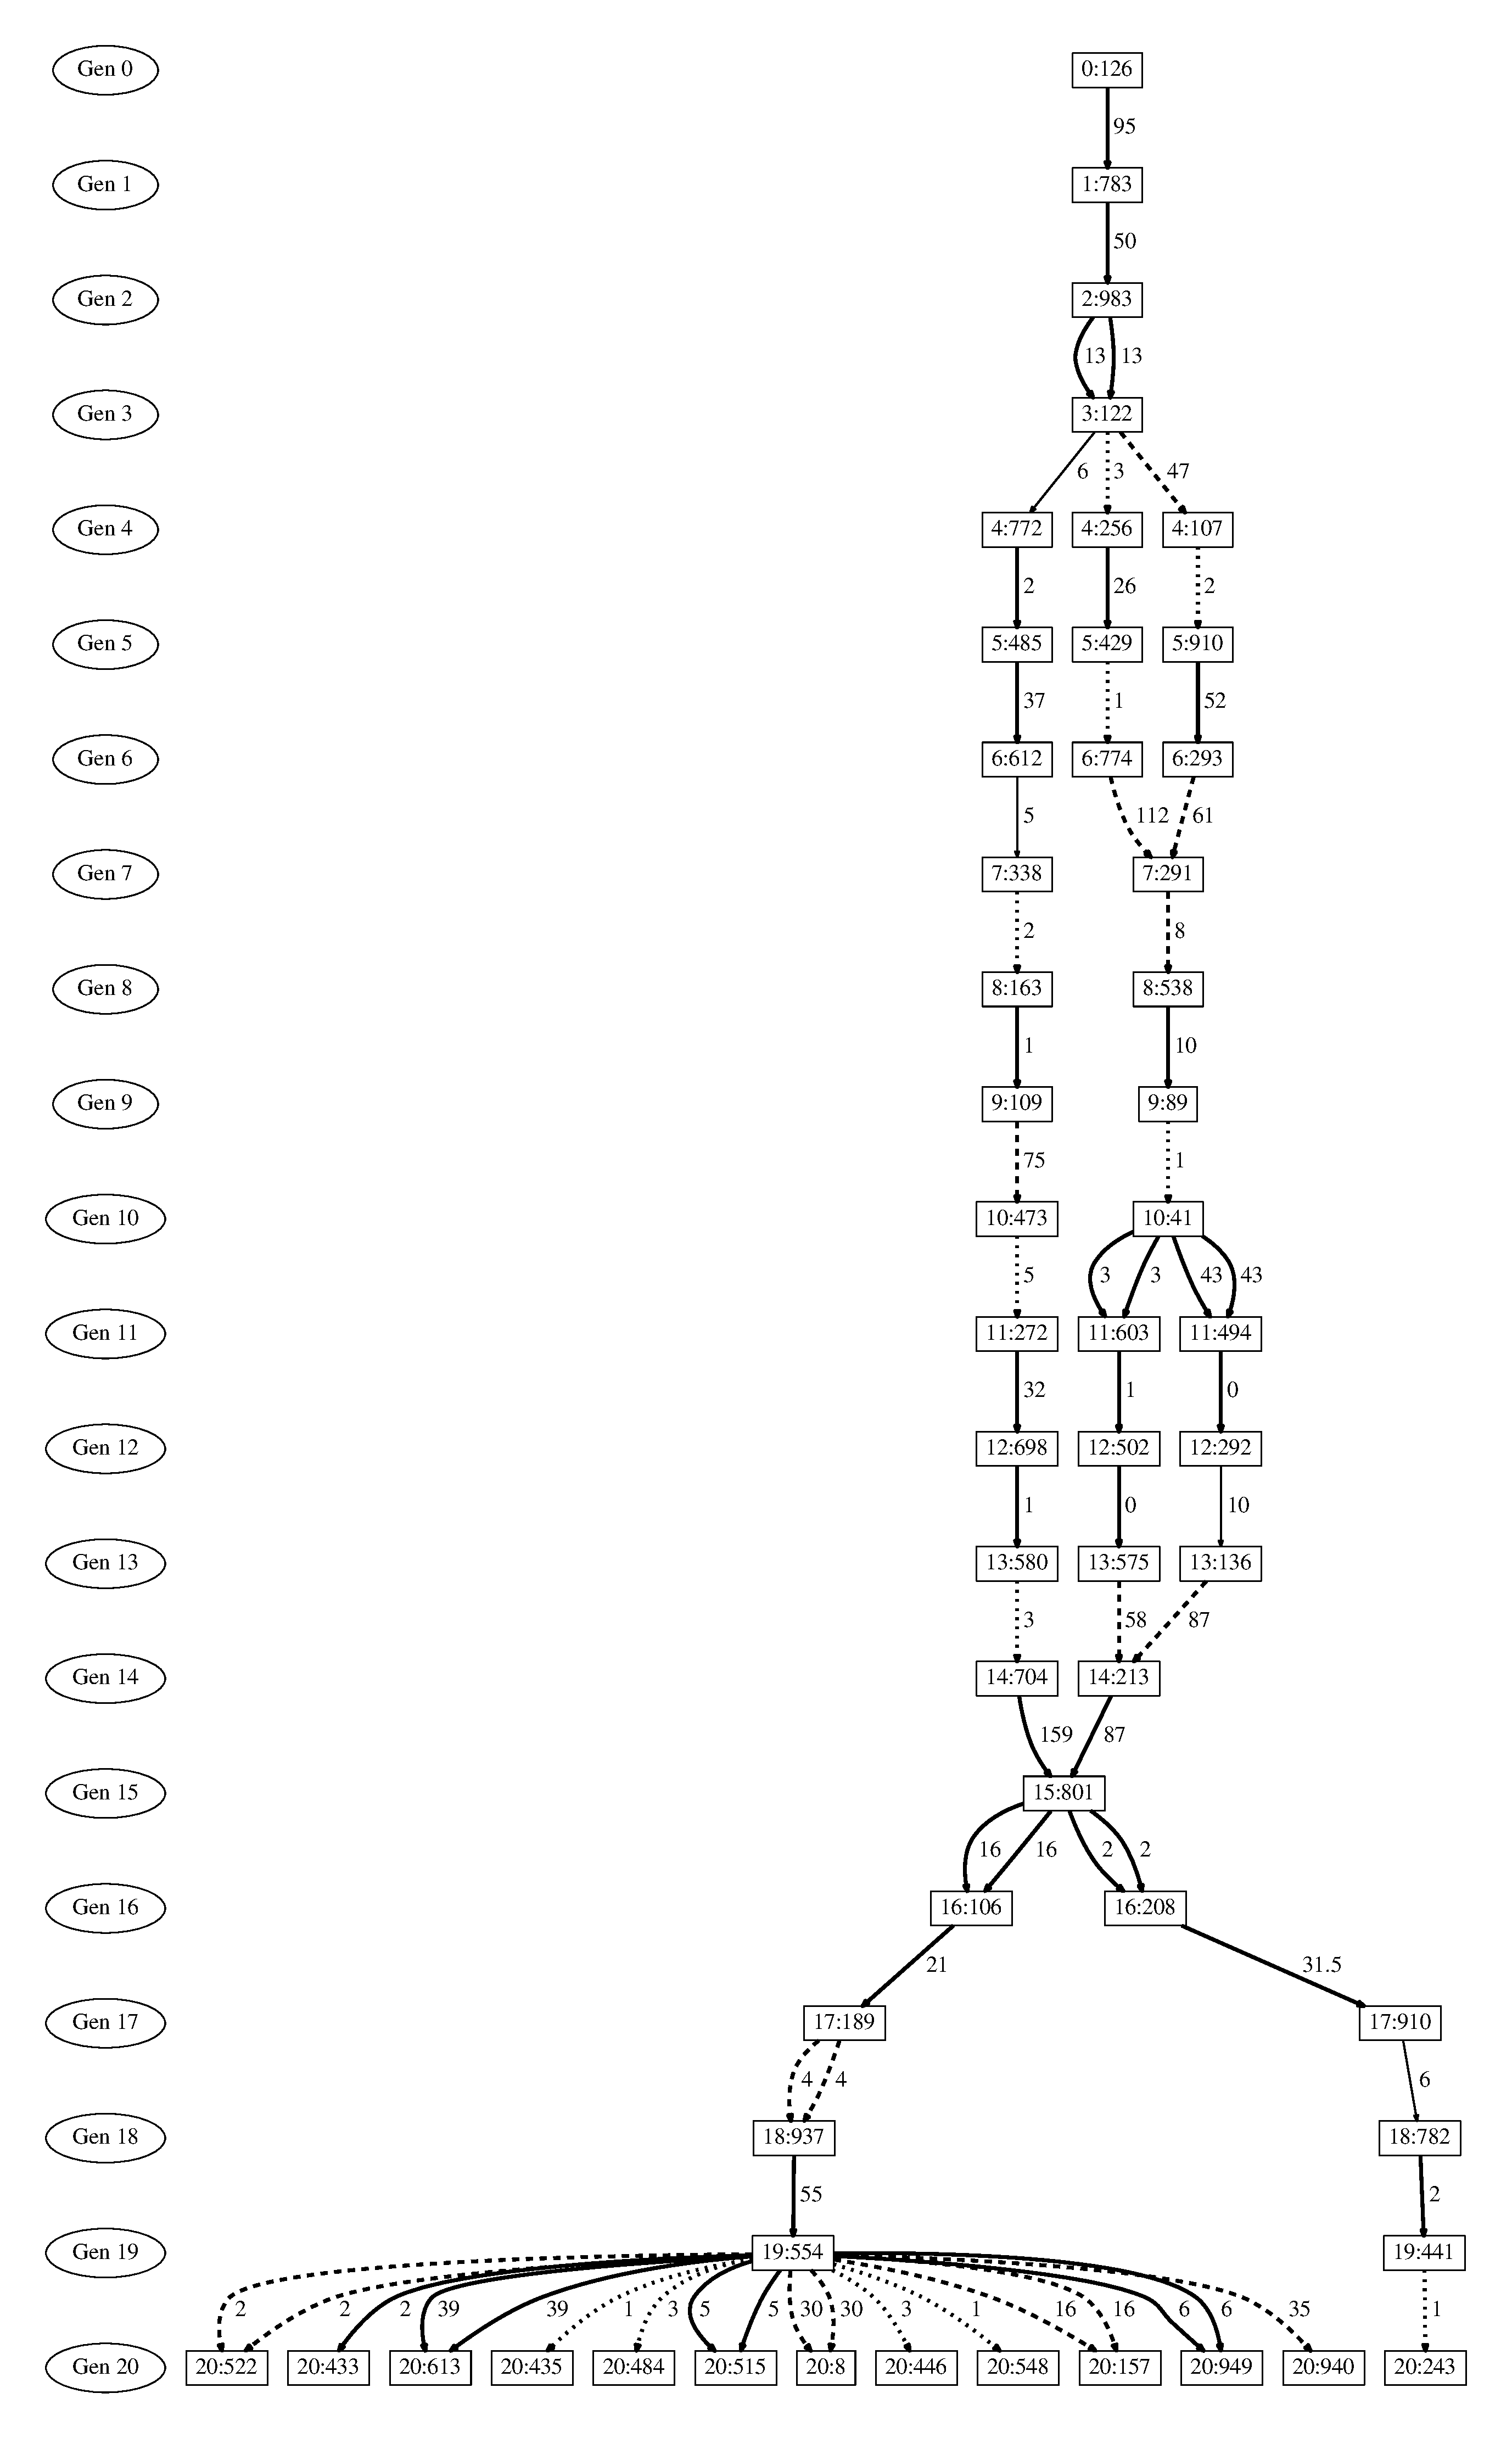
\includegraphics[width=0.9\textwidth]{../figures/run0_GPTP_filtered}
	\end{center}
	\caption{The filtered version of the run's ancestry graph.}
	\label{fig:run0Filtered}       % Give a unique label
\end{figure}

We implemented this filtering by first computing the Damerau-Levenshtein 
distance between genome vectors for each parent-child pair; these distances
are indicated as edge labels in Figure~\ref{fig:run0Filtered}. The genome
vectors were generated by extracting the \texttt{:instruction} and 
\texttt{:close} fields from each gene, and concatenating those into a
single sequence. So, for example, the genome of successful individual
20:484 starts

\todo{Should this prefix of the genome be in a figure so it doesn't
	get broken up by things like page breaks?}
\begin{verbatim}
	{:instruction boolean_and, :close 0} 
	{:instruction boolean_shove, :close 0} 
	{:instruction exec_do*count, :close 0} 
	{:instruction exec_swap, :close 0} 
	{:instruction integer_empty, :close 0}
	...
\end{verbatim}

so the associated genome vector would then be

\begin{verbatim}
	boolean_and 0 boolean_shove 0 exec_do*count 0 
	exec_swap 0 integer_empty 0 ...
\end{verbatim}

Once we had these distances computed, we used it to identify parents in
recombinations that made minimal contributions to the resulting child, so
we could avoid tracing back through those edges, potentially removing not
just that parent, but it's parents, grand-parents, etc. 

Given this distance metric, our filtering algorithm was fairly simplistic.
Assume we have two parents, $p$ and $q$, and a child $c$ such that:
\begin{align*}
	a & = \textrm{DL-distance}(p, c) \\
	b & = \textrm{DL-distance}(q, c) \\
	s & = \textrm{genome-length}(c)
\end{align*}
and assume without loss of generality that $a \leq b$ (i.e., $p$ is the
closer parent). Then we filtered out parent $q$ if either:
\[
	a < 0.2 \times s
\]
or
\[
	b \geq 2 \times a.
\]
Thus parent $q$ will be filtered out if parent $p$ is particularly close to
the child, or if parent $q$ is more than twice as far away from the child as
parent $p$. The choices of the constants $0.2$ and $2$ are obviously somewhat
arbitrary, but appeared to work reasonably well on several datasets. There are,
however, examples where a filtered parent did in fact contribute a significant
number of instructions to the offspring, so one would need to be careful in not
making overly broad assumptions based on an individual not being in the filtered
version of a graph.

\subsection{The (successful) end}

Figure~\ref{prog:simplified20:484} 
\todo{Should the code be in a figure, or just in-lined here in the text? I \emph{think} the figure
	will be closer to the text when more of Section 2 is written. -- NFM}
is the simplified version the successful program from 
individual 20:484. Individual 20:484's genome contains 194 genes, and the unsimplified 
program also contains 194 instructions and passes both
the training and testing cases. The simplified program in 
Figure~\ref{prog:simplified20:484} contains only 9 instructions and
also passes all the tests. 
The simplified program is actually a pretty ``human'' program, and is structured similar to 
how a person might implement replace-space-with-newline using Push. The first five 
instructions (together on the first line) replace all the spaces in the input string 
with newlines (using the \texttt{string\_replacechar} instruction) and print the 
resulting string, thereby solving half the problem. 
The next four instructions (on the second line) remove all the spaces from
a fresh copy of the input string, compute the length and leave that on the
\texttt{:integer} stack as the ``returned'' result.

\begin{figure}[h]
\begin{verbatim}
(\space \newline in1 string_replacechar print_string
 in1 \space string_removechar string_length)
\end{verbatim}
\caption{The simplified version of the successful program from individual 20:484. The
	five instructions on the first line replace all the spaces in the input string with newlines
	and print the result, solving half the problem. The next four instructions (on the second
	line) remove all the spaces from the input string and computing it's length, providing
	the desired ``returned'' result.}
\label{prog:simplified20:484}
\end{figure}

\subsection{How did we get there?}

A few places where we might need to bring in an individual that's 
missing from Figure~\ref{fig:run0Labelled}:
\begin{itemize}
	\item 19:554's other parent
	\item 17:189's other parent
	\item 12:698 and 10:473's other parents.
	\item Maybe 9:89 and 8:538's other parents. Depends somewhat on how much
	they're contributing to the final individual, and whether those 
	contributions are coming from the few changes that come from their other
	parent.
	\item Maybe 6:612, 5:429, and 4:107's other parents. (Same issues as above.)
	\item Maybe 2:983 and 1:783's other parents. If we're running long, though, 
	we could effectively start the process at 2:983 since most everything is
	pretty clean from there down.
\end{itemize}

%\caption{If the width of the figure is less than 7.8 cm use the 
%	\texttt{sidecaption} command to flush the caption on the left side of the 
%	page. If the figure is positioned at the top of the page, align the 
%	sidecaption with the top of the figure -- to achieve this you simply need 
%	to use the optional argument \texttt{[t]} with the \texttt{sidecaption} 
%	command}

\subsection{Creating 15:801: An important crossover}
\label{sec:15:801}

\begin{table}
\begin{tabular}{l|rl|l}
	\textbf{14:704} & & \textbf{15:801} & \textbf{14:213} \\
	\hline
& 1 & & \texttt{(in1} \\ 
\texttt{(\textbackslash space} & 2 & \texttt{(\textbackslash space} & \\ 
\texttt{ \textbackslash newline} & 3 & \texttt{ \textbackslash newline} &  \\ 
& 4 & \texttt{ exec\_dup} &  \\ 
\texttt{ in1} & 4 & \texttt{ in1} &  \\ 
\texttt{ string\_replacechar} & 5 & \texttt{ string\_replacechar} &  \\ 
\texttt{ print\_string} & 6 & \texttt{ print\_string} & \texttt{ print\_string} \\ 
\texttt{ boolean\_stackdepth} & 7 & \texttt{ exec\_dup} & \texttt{ exec\_dup} \\ 
\texttt{ print\_newline)} & 8 &  & \texttt{ exec\_s} \\ 
& 9 &  & \texttt{ (exec\_dup} \\ 
& 10 &  & \texttt{ \ (exec\_rot} \\ 
& 11 & \texttt{ (string\_eq} & \texttt{ \ \ (string\_eq} \\
& 12 & &  \texttt{ \ \ \ string\_fromboolean)} \\ 
& 13 &  & \texttt{ \ \ char\_eq} \\ 
& 14 & & \texttt{ \ \ (string\_emptystring} \\
& 15 & &  \texttt{ \ \ \ boolean\_stackdepth} \\
& 16 & & \texttt{ \ \ \ in1} \\
& 17 & & \texttt{ \ \ \ integer\_gt)} \\ 
& 18 &  & \texttt{ \ \ string\_emptystring} \\ 
& 19 & \texttt{ \ \textbackslash space} & \texttt{ \ \ \textbackslash space} \\ 
& 20 & \texttt{ \ string\_dup} & \texttt{ \ \ string\_dup} \\ 
& 21 & \texttt{ \ string\_removechar} & \texttt{ \ \ string\_removechar} \\ 
& 22 & \texttt{ \ string\_rot} & \texttt{ \ \ boolean\_pop} \\ 
& 23 &   & \texttt{ \ \ in1} \\ 
& 24 &   & \texttt{ \ \ string\_butlast} \\ 
& 25 &   & \texttt{ \ \ string\_last} \\ 
& 26 &   & \texttt{ \ \ string\_parse\_to\_chars} \\
& 27 &   & \texttt{ \ \ exec\_when} \\ 
& 28 &   & \texttt{ \ \ string\_dup} \\
& 29 &   & \texttt{ \ \ string\_removechar} \\
& 30 & \texttt{ \ string\_last} & \texttt{ \ \ string\_last} \\
& 31 & \texttt{ \ string\_parse\_to\_chars} & \texttt{ \ \ string\_parse\_to\_chars} \\
& 32 & \texttt{ \ string\_rot)} & \texttt{ \ \ string\_rot)} \\
& 33 & \texttt{ in1} & \texttt{ \ in1)} \\
& 34 & \texttt{ string\_stackdepth)} & \texttt{ string\_stackdepth)} \\
\end{tabular}
\caption{The details of the recombination event (alternation followed by
	uniform mutation) that created individual
	15:801 (center) from parents 14:704 (left) and 14:213 (right) showing
	the \emph{simplified} programs for those individuals (see
	Section~\ref{sec:background}). This shows that individual 15:801 was
	essentially constructed from a prefix of 14:704 and a suffix of 14:213.
	See Section~\ref{sec:15:801} for additional details.}
\label{tab:15:801}
\end{table}

\section{Discussion}
\label{sec:discussion}

Wrap up with some kind of ``big picture'' that does things like catalogs the
\emph{kinds} of operations, their frequency, etc.


% \paragraph{Paragraph Heading} %



% \subparagraph{Subparagraph Heading} In order to avoid simply listing headings of different levels we recommend to let every heading be followed by at least a short passage of text. Use the \LaTeX\ automatism for all your cross-references and citations as has already been described in Sect.~\ref{sec:2}, see also Fig.~\ref{fig:2}.

% Use the \index{} command to code your index words
% Make sure to inlcude the indexed word inside and outside of the brackets if you want the text to show up in your paragraph:
% e.g. This book is about \index{genetic programming}genetic programming. 
% If the text is not entered outside the brackets it will appear as: This book is about .

\section{Conclusions}
\label{sec:conclusions}

We did it! Yay! Oh, and it was useful and matters in some way.

\begin{acknowledgement}
	Emma Sax, Laverne Schrock, and Leonid Scott helped 
	with the initial computation and analyses of the differences between the 
	parents and children discussed here. William Tozier provided a host of 
	ideas and feedback all through the process.
\end{acknowledgement}

\bibliographystyle{spbasic}
\bibliography{gp-bibliography,chapter}
